\documentclass[11pt,letterpaper,titlepage]{article}

\usepackage{geometry}
\geometry{left=2cm,right=2cm,top=2cm,bottom=3cm}

\usepackage{setspace}
\onehalfspacing

\usepackage{multicol}
\setlength{\columnsep}{3em}

\usepackage{booktabs}

\usepackage[table,x11names]{xcolor}

\usepackage{multirow}

\usepackage{pgfgantt}

\usepackage{listings}

\usepackage{xcolor}
\definecolor{vgreen}{RGB}{104,180,104}
\definecolor{vblue}{RGB}{49,49,255}
\definecolor{vorange}{RGB}{255,143,102}

\lstdefinestyle{verilog-style}
{
    language=Verilog,
    basicstyle=\small\ttfamily,
    keywordstyle=\color{vblue},
    identifierstyle=\color{black},
    commentstyle=\color{vgreen},
    % numbers=left,
    numberstyle=\tiny\color{black},
    numbersep=11pt,
    tabsize=4,
    moredelim=*[s][\colorIndex]{[}{]},
    literate=*{:}{:}1
}

\lstdefinestyle{txt-style}
{
    basicstyle=\small\ttfamily,
    % numbers=left,
    numbersep=11pt,
    tabsize=4,
    moredelim=*[s][\colorIndex]{[}{]},
    literate=*{:}{:}1
}

\usepackage{tikz}
\usetikzlibrary{shapes.geometric, arrows, positioning, fit,calc}
\newcommand*\circled[1]{\tikz[baseline=(char.base)]{
            \node[shape=circle,draw,inner sep=1pt] (char) {#1};}}
            
\usepackage{hyperref}
\hypersetup{
    colorlinks,
    citecolor=black,
    filecolor=black,
    linkcolor=black,
    urlcolor=black
}

\usepackage{pifont}

\usepackage[toc,page]{appendix}

\pagestyle{empty}
\usepackage{tikz}
\usetikzlibrary{shapes.geometric, arrows}

\usetikzlibrary{mindmap,trees}
\usepackage{verbatim}

\usepackage{indentfirst}
\setlength{\parindent}{2em}

\usepackage{listings}

% \usepackage{hyperref}
\usepackage{chngcntr}
\counterwithin{section}{part}
\renewcommand\thesection{\arabic{section}}

\usepackage{graphicx}

\usepackage{subcaption}

\usepackage{fancyhdr}

\pagestyle{fancy}
\lhead{}
\rhead{}
\lfoot{ECEN 749 Lab 1}
\cfoot{\thepage}
\rfoot{@Lei Wang (Wilson)}
\renewcommand{\headrulewidth}{0pt}
\renewcommand{\headwidth}{\textwidth}
\renewcommand{\footrulewidth}{0.4pt}
\newcommand{\RomanNumeralCaps}[1]
    {\MakeUppercase{\romannumeral #1}}

\makeatletter
\newcommand*\@lbracket{[}
\newcommand*\@rbracket{]}
\newcommand*\@colon{:}
\newcommand*\colorIndex{%
    \edef\@temp{\the\lst@token}%
    \ifx\@temp\@lbracket \color{black}%
    \else\ifx\@temp\@rbracket \color{black}%
    \else\ifx\@temp\@colon \color{black}%
    \else \color{vorange}%
    \fi\fi\fi
}
\makeatother

\usepackage{trace}

\begin{document}

\begin{titlepage}
  \centering
	{\scshape\large Texas A\&M University \par}
	\vspace{1cm}
	{\scshape\Large Department of Electrical and Computer Engineering \par}
	\vspace{4cm}
    \vspace{0.5cm}
	{\huge\bfseries ECEN 749 Microprocessor System Design\par}
	\vspace{4cm}
	{\Large Lab 1 Report (Section 601)\par}
	\vspace{1cm}
	{\Large Student: Lei Wang (Wilson)\par}
	\vspace{1cm}
	{\Large UIN: 829009485\par}
	\vspace{1cm}
	{\Large Instructor: Dr. Paul V. Gratz\par}
	\vspace{4cm}
	\vfill

  % Bottom of the page
	{\large Submitted: Janauary 21th, 2020 \par}

\end{titlepage}

\newpage

\tableofcontents{}

\newpage

\part{Introduction}

The first lab session of ECEN 749 aims to familiarize the students with basic operations using the \textit{Zybo Z7-20: Zynq-7000 ARM/FPGA SoC Development Board} and to refresh students' memory on Verilog HDL. The lab uses \textit{Xilinx Vivado 2015.2} as the development tool for generating bitstream and communicating with the FPGA board.

\begin{table}[ht]
\centering
\begin{tabular}{@{}cl@{}}
\toprule
Experiment & Description                                           \\ \midrule
1          & Implement a switch-operated LED array                 \\
\midrule
2          & Implement a button-controlled counter                 \\
\midrule
3          & Implement the jackpot game with indication on winning \\ \bottomrule
\end{tabular}
\caption{Experiments for the first lab session.}
\end{table}

The lab consists of three experiments with increasing levels of difficulty. Only the first experiment comes with detailed instructions. The procedures and outcomes are outlined in the later chapters.

\part{Procedure}

\section{Switch-Operated LED Array}

\begin{enumerate}
    \item Setup the environment for Vivado by running the following command in terminal:
    
    \verb|source /opt/coe/Xilinx/Vivado/2015.2/settings64.sh|
    
    \item Run the following command to launch Vivado:
    
    \verb|vivado|
    
    \item Click on \textbf{File} $\rightarrow$ \textbf{Create New Project} to open the dialog window.
    
    \item Enter the project name \textbf{``lab1\_1\_LED''} and choose a location to store the project files. Click on \textbf{``Next''}.
    
    \item Select \textbf{``RTL project''}. Uncheck \textbf{``Do not specify sources''}. Click on \textbf{``Next''}.
    
    \item Select \textbf{``Verilog''} as the \textbf{``Target language''}. Select \textbf{``Mixed''} as the \textbf{``Simulator language''}. Click on \textbf{``Next''}.
    
    \item Click on the \textbf{``+''} mark. Select \textbf{``Create file''}.
    
    \item In the pop-up window, call it \textbf{``switch''} in the \textbf{``File name''} field. Keep the \textbf{``File location''} option as \textbf{``$<$local to project$>$''}. Click on \textbf{``OK''} to close the windows.
    
    \item Click on \textbf{``Next''} to skip the process of adding any existing IP.
    
    \item Click on \textbf{``Next''} to skip the processing of adding any constraint.
    
    \item Click on \textbf{``Parts''} in the \textbf{Default Part} window. Select the following components. Then click on \textbf{``Next''}.
    
    \begin{table}[ht]
    \centering
    \begin{tabular}{@{}ll@{}}
    \toprule
    Product Category & All             \\ \midrule
    Family           & Zynq-7000       \\ \midrule
    Sub-Family       & Zynq-7000       \\ \midrule
    Package          & clg400          \\ \midrule
    Speed grade      & -1              \\ \midrule
    Temp garde       & All Remaining   \\ \midrule
    Part             & xc7z010clg400-1 \\ \bottomrule
    \end{tabular}
    \caption{Select the device when creating.}
    \end{table}
    
    \item Click on \textbf{``Finish''} to create the project.
    
    \item In the \textbf{Define Module} window, enter \textbf{``switch''} in the \textbf{Module name} field and enter the following information:
    
    \begin{table}[ht]
    \centering
    \begin{tabular}{@{}lllll@{}}
    \toprule
    Port Name & Direction & Bus & MSB & LSB \\ \midrule
    SWITCHES  & input     & \ding{52} & 3   & 0   \\ \midrule
    LEDS      & output    & \ding{52} & 3   & 0   \\ \bottomrule
    \end{tabular}
    \caption{Define module.}
    \end{table}
    
    \item A text editor field with name \textbf{switch.v} should appear, if not, click on \textbf{Flow} $\rightarrow$ \textbf{Project Manager} to open the view, then select \textbf{``switch.v''} to open the text editor. The 
    
    \item Copy and paste the code in Appendix \ref{appendix:verilog_switch} into the text editor. Remember to save the code.
    
    \item Create a file called \textbf{switch.xdc} (see Appendix \ref{appendix:xdc_switch}). Place the \textit{.xdc} file into the project by right click on the \textbf{Constraints} folder in the \textbf{Source} window $\rightarrow$ \textbf{Add or create constraints} $\rightarrow$ \textbf{Next} $\rightarrow$ \textbf{$+$} $\rightarrow$ \textbf{Add files} $\rightarrow$ select the \textit{.xdc} file $\rightarrow$ \textbf{OK}. 
    
    \item After selecting the \textbf{switch.v} file in the \textbf{Source} panel, click on \textbf{Generate Bitstream} under the \textbf{PROGRAM AND DEBUG} tab from the \textbf{Flow Navigator} panel. Click \textbf{Yes} if there were any warnings.
    
    \item Set the jumper \textbf{JP5} on the FPGA board to \textbf{JTAG}.
    
    \item Connect the power adaptor to the wall plug and the FPGA board. Flip on the power switch on the FPGA board.
    
    \item Click on \textbf{Open Hardware Manager} under the \textbf{PROGRAM AND DEBUG} tab from the \textbf{Flow Navigator} panel.
    
    \item In the \textbf{HARDWARE MANAGER} panel, click \textbf{Open target} $\rightarrow$ \textbf{Auto Connect}. The FPGA board information should appear in the \textbf{Hardware} tab under the \textbf{HARDWARE MANAGER} the panel.
    
    \item Click \textbf{Program Device} under the \textbf{PROGRAM AND DEBUG} tab in the \textbf{Flow Navigator} panel. Select the FPGA board as the target device. Click \textbf{Program}.
    
    \item Toggle the switches to see the effect of switching on and off the LEDs.
    
\end{enumerate}

\section{Button-Controlled Counter}

Procedures for this experiment is the same as those for the previous experiment, except the following:

\begin{enumerate}
    \item Project is named as \textbf{Counter}.
    
    % \item define module difference should be addressed here.
    
    % \item code: the counter.v file
    
    % \item code: the counter.xdc file.
    
    % list the names of the switches
    
    \item To see the effect, keep pressing one of the two switches and notice the LEDs are acting as a counter displaying binary numbers. The period is approximately one second.
    
    % explain how to achieve the exactly one second counting period here.
    
\end{enumerate}

\section{Jackpot Game}

Procedures for this experiment is the same as those for the first experiment, except the following:

\begin{enumerate}
    \item Project is named as \textbf{Counter}.
    
    \item
    
      % \item define module difference should be addressed here.
    
    % \item code: the counter.v file
    
    % \item code: the counter.xdc file.
    
    % list the names of the switches
    
    \item To see the effect, flip on the switch that is directly below the LED that is on. All LEDs should start flashing at the same time if the correct switch is toggled.
    
    % explain the period used here
    
\end{enumerate}

\newpage

\part{Results}

\section{Switch-Operated LED Array}

The outcome is as expected. When flipping the switch, an LED corresponding to that particular switch lights on and off as the switch is turned on and off. Lighting up multiple LEDs is possible and each switch does not interfere with the operation other switches and LEDs.

% add a picture here

% add the simulation results here

\section{Button-Controlled Counter}

% specify the names of the buttons here

% double check the conditions, i.e. down-counting from 0 will not result in 1111

The outcome is as expected. When pressing the button for up counter, the binary number represented by the LEDs counts up and vice versa. When the LEDs are all on, representing a binary number of 0'b1111, pressing the up-counting button results in a counting cycle starting from 0. The counter has a capacity of 4 bits and when it overflows, it restarts from 0. When all the LEDs are off, representing a binary number of 0'b0000, pressing the down-counting button will not switch on or off any LEDs. Down-counting from 0 yields 0.

\section{Jackpot Game}

% alter the speed of the one-hot fashion switching of the LEDs

The outcome is as expected. The LEDs are switched on and off in one-hot fashion at a constant interval. When all LEDs are switched on once, a new cycle starts from the first LED that is switched on. While LEDs are being switch on and off, flipping the switch that corresponds to the on-state LED ends the game. After the game ends, all LEDs are turned on and off at the same time, indicating a winning situation has been reached. Flipping the switch after winning the game does not change anything. The player cannot win the game by turning on multiple switches.

\newpage

\part{Conclusion}

From this lab session, I have learned how to use the \textbf{Xilinx Vivado} design suite to make hardware design and run the design on a FPGA board. I have refreshed my memory on writing Verilog by doing those three experiments.

My approach was primarily based on a software-programming perspective instead of the hardware way. Each piece of Verilog code should correspond to hardware blocks that can be manufactured. Hence I ran into some issues like not using \textbf{reg} in an \textbf{always} block. Thinking from a software perspective works for this lab session but may expose vulnerabilities when it comes to large and complex hardware design. 

Q: How are the user push-buttons wired on the ZYBO Z7-10 board?

A: According to \href{https://reference.digilentinc.com/reference/programmable-logic/zybo-z7/reference-manual}{https://reference.digilentinc.com/reference/programmable-logic/zybo-z7/reference-manual}:

% change the picture to a table, remove the picture, including information regarding whether it is pull-up or pull-down switches.

\begin{figure}[ht]
\centering
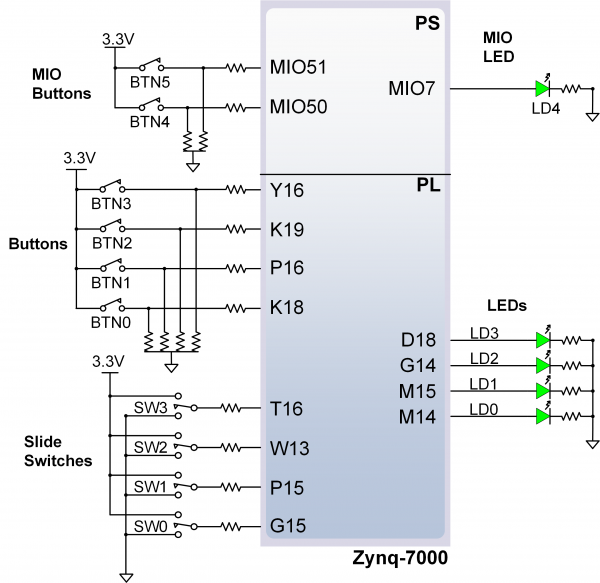
\includegraphics[width=0.6\textwidth]{zybo-z7-gpio.png}
\caption{Pin layout for the buttons and switches on Zybo-Z7 board.}
\end{figure}

Edit the \textit{.xdc} file in the following format:

\lstinputlisting[style={txt-style}]{xdc.txt}

Q: What is the purpose of an edge detection circuit and how should it have been used in this lab?

A: An edge detection circuit generates a pulse signal when its input waveform is rising or falling. The edge detector circult can be used in the counter design. In my code, there are multiple places where the \textbf{posedge} keyword is used when writing the \textbf{always} block. The edge detection circuit can be used when connecting the clock and the counter circuit, or as the connection between the counter and the jackpot circuit.

\newpage

\begin{appendices}

\section{switch.v}
\label{appendix:verilog_switch}
\lstinputlisting[style={verilog-style}]{switch.v}

\section{switch.xdc}
\label{appendix:xdc_switch}
\lstinputlisting[style={txt-style}]{switch_xdc.txt}

\end{appendices} 

% place the code and the xdc files here for the second and the third experiment.

\end{document}